
%----------------------------------------------------------------------------------------
%	PACKAGES AND DOCUMENT CONFIGURATIONS
%----------------------------------------------------------------------------------------

\documentclass{scrartcl}

\usepackage{siunitx} % Provides the \SI{}{} command for typesetting SI units
\usepackage{booktabs}

\usepackage{hyperref}
\usepackage{xspace}

\usepackage{graphicx} % Required for the inclusion of images
\usepackage{listings}
\setlength\parindent{0pt} % Removes all indentation from paragraphs

\renewcommand{\labelenumi}{\alph{enumi}.} % Make numbering in the enumerate environment by letter rather than number (e.g. section 6)

%----------------------------------------------------------------------------------------
%	DOCUMENT INFORMATION
%----------------------------------------------------------------------------------------

\def\pxar {{pXar}\xspace}

\def\cmake {{\tt cmake}\xspace}

\newcommand{\fixme[1]} {\textcolor{red}{FIXME: #1}\xspace}

\def\testparameters {{\tt testparameters.dat}\xspace}

\def\usertests {{\tt pxar/usertests}\xspace}

\def\fulltest {{\tt FullTest}\xspace}
\def\pretest {{\tt PreTest}\xspace}
\def\alivetest {{\tt PixelAliveTest}\xspace}
\def\masktest {{\tt MaskTest}\xspace}
\def\bbtest {{\tt BumpBondingTest}\xspace}
\def\trimming {{\tt Trimming}\xspace}
\def\trimbits {{\tt TrimBitsTest}\xspace}
\def\phcalibration {{\tt PulseHeightCalibration}\xspace}
\def\scurves {{\tt sCurveTest}\xspace}
\def\thrMaps {{\tt ThresholdTest}\xspace}
\def\hrmaps {{\tt HighRateTest}\xspace}

\def\dac {{\tt DAC}\xspace}
\def\dacs {{\tt DACs}\xspace}

\def\roc {{ROC}\xspace}
\def\ph {{pulse height}\xspace}





\title{pxar User Manual} % Title

\author{
} % Author names

\date{\today} % Date for the report

\begin{document}

\maketitle % Insert the title, author and date


\begin{abstract}
The goal of this document is to provide a user manual for operation of
PSI46 Chips and Modules with the Digital Testboard (DTB).
\end{abstract}

\newpage
% Table Of Contents
\tableofcontents

\newpage

% ----------------------------------------------------------------------
\section{Introduction}
\label{s:introduction}
% ----------------------------------------------------------------------

% ----------------------------------------------------------------------
\section{Hardware overview}
\label{s:hwOverview}
% ----------------------------------------------------------------------

% ======================================================================
\section{Software design overview}
\label{s:swOverview}
% ======================================================================

% ----------------------------------------------------------------------
\subsection{API and hardware abstraction layer}
\label{ss:core}



% ----------------------------------------------------------------------
\subsection{User interface and tests}
\label{ss:ui}


% ======================================================================
\section{Tutorial}
\label{s:tutorial}
% ======================================================================

If you encounter any problems that you cannot solve, please check in 
\url{https://twiki.cern.ch/twiki/bin/viewauth/CMS/Pxar#FAQ} for a
similar problem and solution, post a question to
\href{https://hypernews.cern.ch/HyperNews/CMS/get/pixel-psi46-testboard.html}{\tt
  pixel-psi46-testboard hypernews}, or open an issue at \url{https://github.com/psi46/pxar/issues/new}.

% ----------------------------------------------------------------------
\subsection{Installation}
\label{ss:installation}

You need the following packages/programs on your computer: 
\begin{itemize}
  \item C++ compiler
  \item ROOT 5.34/xx. Do not attempt to use ROOT 5.99, the
    beta-release of ROOT 6, as it will not work. 
  \item git
  \item cmake
  \item USB (header files)
  \item FTDI drivers
\end{itemize}
\fixme[add much more details. Volunteers?!]

% ----------------------------------------------------------------------
\subsection{Setup}
\label{ss:setup}
The \pxar code is hosted at \url{https://github.com/psi46/pxar}. Get it with 
{\tt
\begin{verbatim}
git clone git@github.com:psi46/pxar 
cd pxar
mkdir build
\end{verbatim}
}
If you run into problems here, you likely should setup git correctly
(see section~\ref{ss:installation}). 

For the time being, it is recommended that you get the HEAD of the
master branch. 


% ----------------------------------------------------------------------
\subsection{Compilation}
\label{ss:compilation}
Assuming that you start from the {\tt pxar} directory, do
{\tt
\begin{verbatim}
cd build
cmake -DBUILD_pxarui=ON ..
make [-j4] install [VERBOSE=1]
\begin{verbatim}
}
This will install by default the library into pxar/lib and the
executables into pxar/bin 
(both directories are subfolders of your local pxar folder).

Other cmake build options include
{\tt
\begin{verbatim}
cmake -DBUILD_pxarui=OFF ..
cmake -DBUILD_dummydtb=ON ..
\end{verbatim}
}

% ----------------------------------------------------------------------
\subsection{DTB firmware}
\label{ss:firmware}


To properly operated the DTB, you also need to have the matching
firmware loaded onto that device. The firmware can be obtained from 
\url{https://github.com/psi46/pixel-dtb-firmware/tree/master/FLASH} and the loaded
onto the DTB (its FPGA) with the following statements (assuming that
you are in directory {\tt pxar}): 
{\tt
\begin{verbatim}
cd ..
git clone git@github.com:psi46/pixel-dtb-firmware.git
cd pxar/main
../bin/pXar -f ../../pixel-dtb-firmware/FLASH/FLASHFILE
\end{verbatim}
} 
where {\tt FLASHFILE} should be replaced with the name of the most
recent version. The download will take a while. Follow the
instructions at the end: Wait until all 4 LEDs turn off and
power-cycle the DTB.

% ----------------------------------------------------------------------
\subsection{Program execution}
\label{ss:run}
The simplest way to run something of the \pxar framework is to use the
standalone test program: 
{\tt
\begin{verbatim}
../bin/testpxar
\end{verbatim}
}

To run the GUI, do 
{\tt
\begin{verbatim}
../bin/pXar -d ../data/defaultParametersRocPSI46digV2 -g [-v WARNING|QUIET|...]
../bin/pXar -d ../data/defaultParametersModulePSI46digV2 -g [-v WARNING|QUIET|...]
\end{verbatim}
}

and without the GUI, using a 'standard' ROOT C++ macro
{\tt
\begin{verbatim}
../bin/pXar -d ../data/defaultParametersRocPSI46digV2 \
  -c '../scripts/singleTest.C("DacScan", "DacScan.root")'
\end{verbatim}
}
% ======================================================================
\section{Tests}
\label{s:tests}
% ======================================================================


% ----------------------------------------------------------------------
\subsection{FullTest}
\label{ss:fulltest}

The suite of tests that is run to qualify pixel modules is called
\fulltest. It is a sequential test suite that is run multiple times at
different temperatures. It is composed of the following tests, which
are described in more detail in the following sections.

\begin{table}[!htb]
  \caption{Overview of all tests implemented in \pxar. The order of
    the tests in this table does not correspond to their arrangement
    in \pxar, but rather to their relevance. Notes:
  In \testparameters, the test name appears without {\tt `Test'}. Test
  entries marked with (*) are contained in the {\tt doTest} entry of
  the corresponding test.}  \label{t:testoverview}
  \vspace*{0.5cm}
  \begin{scriptsize}
  \begin{tabular}{|l|l|l|l|} \hline
    {\bf Test name}   &{\bf Entry } &{\bf Type} & {\bf Description}  \\
    \hline
    \pretest   &{\tt programroc}  (*)     &basic test          &ROCs can be programmed?\\
               &{\tt setvana}       (*)   &configuration       &basic configuration\\
               &{\tt setvthrcompcaldel} (*)&configuration      &basic configuration\\
               &{\tt settimings}      &configuration       &configure timing for TBM08A/TBM08B   \\
               &{\tt findtimings}   (*)   &configuration       &configure timing for $>$TBM08B   \\
               &{\tt findWorkingPixel} (*)&functionality       &same working pixel in all ROCs\\
    \hline
    \alivetest &{\tt alivetest}  (*)      &functionality       &test response of pixels\\
               &{\tt masktest}    (*)     &functionality &test masking of pixels\\
               &{\tt addressdecodingtest} (*) &functionality  &test address of pixels\\
    \hline
    \trimtest  &{\tt trim}       (*)  &optimization       &unify pixel thresholds\\
               &{\tt trimbits}  (*)   &functionality      &test trim bits\\
    \hline
    \phtest    &{\tt optimize} (*)    &optimization       &ensure maximum usage of ADC range\\
               &{\tt phmap}           &characterization   &measure 2D \ph\ map\\
    \hline
    \gptest    &{\tt measure} (*)     &optimization       &measure \ph\ vs.~\vcal\\
               &{\tt fit}  (*)        &optimization       &parametrize \ph\ vs.~\vcal\\
    \hline
    \bbtest    &{\tt dotest}          &functionality      &test bump bond connectivity\\
    \hline
\end{tabular}
\end{scriptsize}
\end{table}


% ----------------------------------------------------------------------
\subsection{Pretest}
\label{ss:pretest}

% ----------------------------------------------------------------------
\subsection{PixelAlive test}
\label{ss:alivetest}

% ----------------------------------------------------------------------
\subsection{Mask bit test}
\label{ss:masktest}

% ----------------------------------------------------------------------
\subsection{Bump bonding test}
\label{ss:bbtest}

% ----------------------------------------------------------------------
\subsection{Trimbits test}
\label{ss:trimbits}

% ----------------------------------------------------------------------
\subsection{Trimming}
\label{ss:trimming}

% ----------------------------------------------------------------------
\subsection{S-curves}
\label{ss:scurves}

% ----------------------------------------------------------------------
\subsection{Threshold maps}
\label{ss:thrmaps}


% ----------------------------------------------------------------------
\subsection{\Ph\ optimization}
\label{ss:phopt}

The analog pixel signal is digitized in the \roc\ periphery. The
amplitude of the resulting digital ADC signal is referred to as \ph.

The purpose of the {\tt\phtest:optimize} test is to ensure that small
signals are output with small ADC values and that large signals are
output with large ADC values in such a way that the largest possible
ADC range is used. This is achieved by tuning the \dac\ parameters
\phoffset\ and \phscale. The basic idea behind the algorithm is to
maximize the range (difference between the \ph\ of large signals and
small signals).

The test proceeds by determining, per ROC, the pixels with the lowest
(highest) \ph\ for a charge injection corresponding to \vcal = 10
(255), in the high range. This step is required because the
\ph\ distribution shows a significant pixel-to-pixel variation, as
shown in Fig.~\ref{f:phmap}. If a random pixel were chosen for the
optimization, saturation (at the low and high end) would affect the
\ph\ distribution.

\begin{figure}[!htb]
 \begin{centering}
  \unitlength1.0cm % coordinates in cm
  \begin{picture}(15.0,6.)
    \put(2.5, 0.){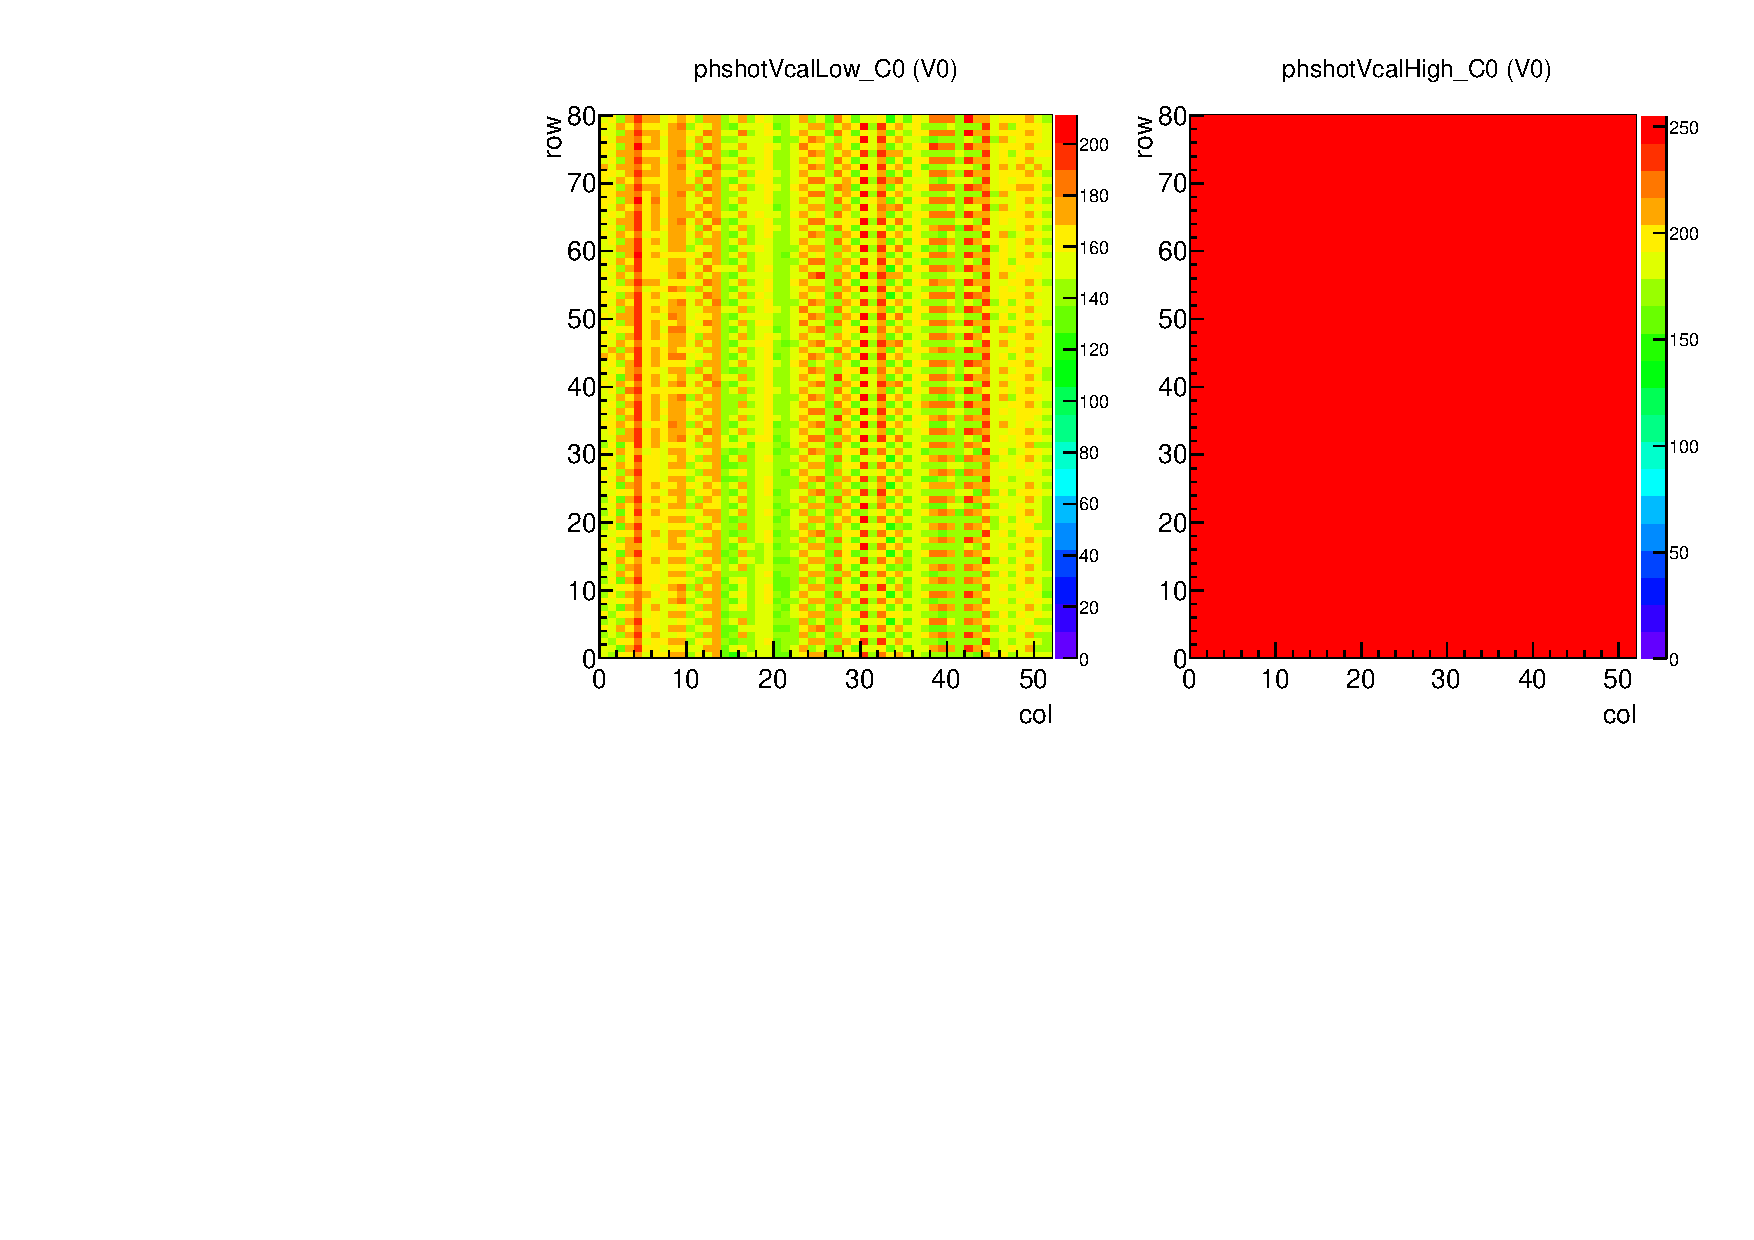
\includegraphics[height=6cm]{../doc/usermanual/fig/ph-loshot-hishot-default.pdf}}
  \end{picture}
  \caption{\Ph\ map, before \phscale\ and \phoffset\ optimization, for
    \vcal=10 (left) and \vcal=255 (right), in the high range. The
    significant \ph\ variation for the low-\vcal\ injection is visible in the left plot, and the
    saturation for the large-\vcal\ injection is evident in the right
    plot.}
  \label{f:phmap}
 \end{centering}
\end{figure}



The two \dac\ parameters \phoffset\ and \phscale\ are scanned for a
low and high \vcal\ value (in the high range) for the two pixels (the
pixel with the lowest PH for the low-\vcal\ injection and the pixel
with the highest PH for the high-\vcal\ injection). The two 2D
distributions of the high-PH and the low-PH values are subtracted and
the optimal setup is chosen as that (\phoffset, \phscale) point which
maximizes the range. These three steps are illustrated in
Fig.~\ref{f:phoptillustration}.


\begin{figure}[!htb]
 \begin{centering}
  \unitlength1.0cm % coordinates in cm
  \begin{picture}(15.0,6.0)
    \put(0.5, 0.){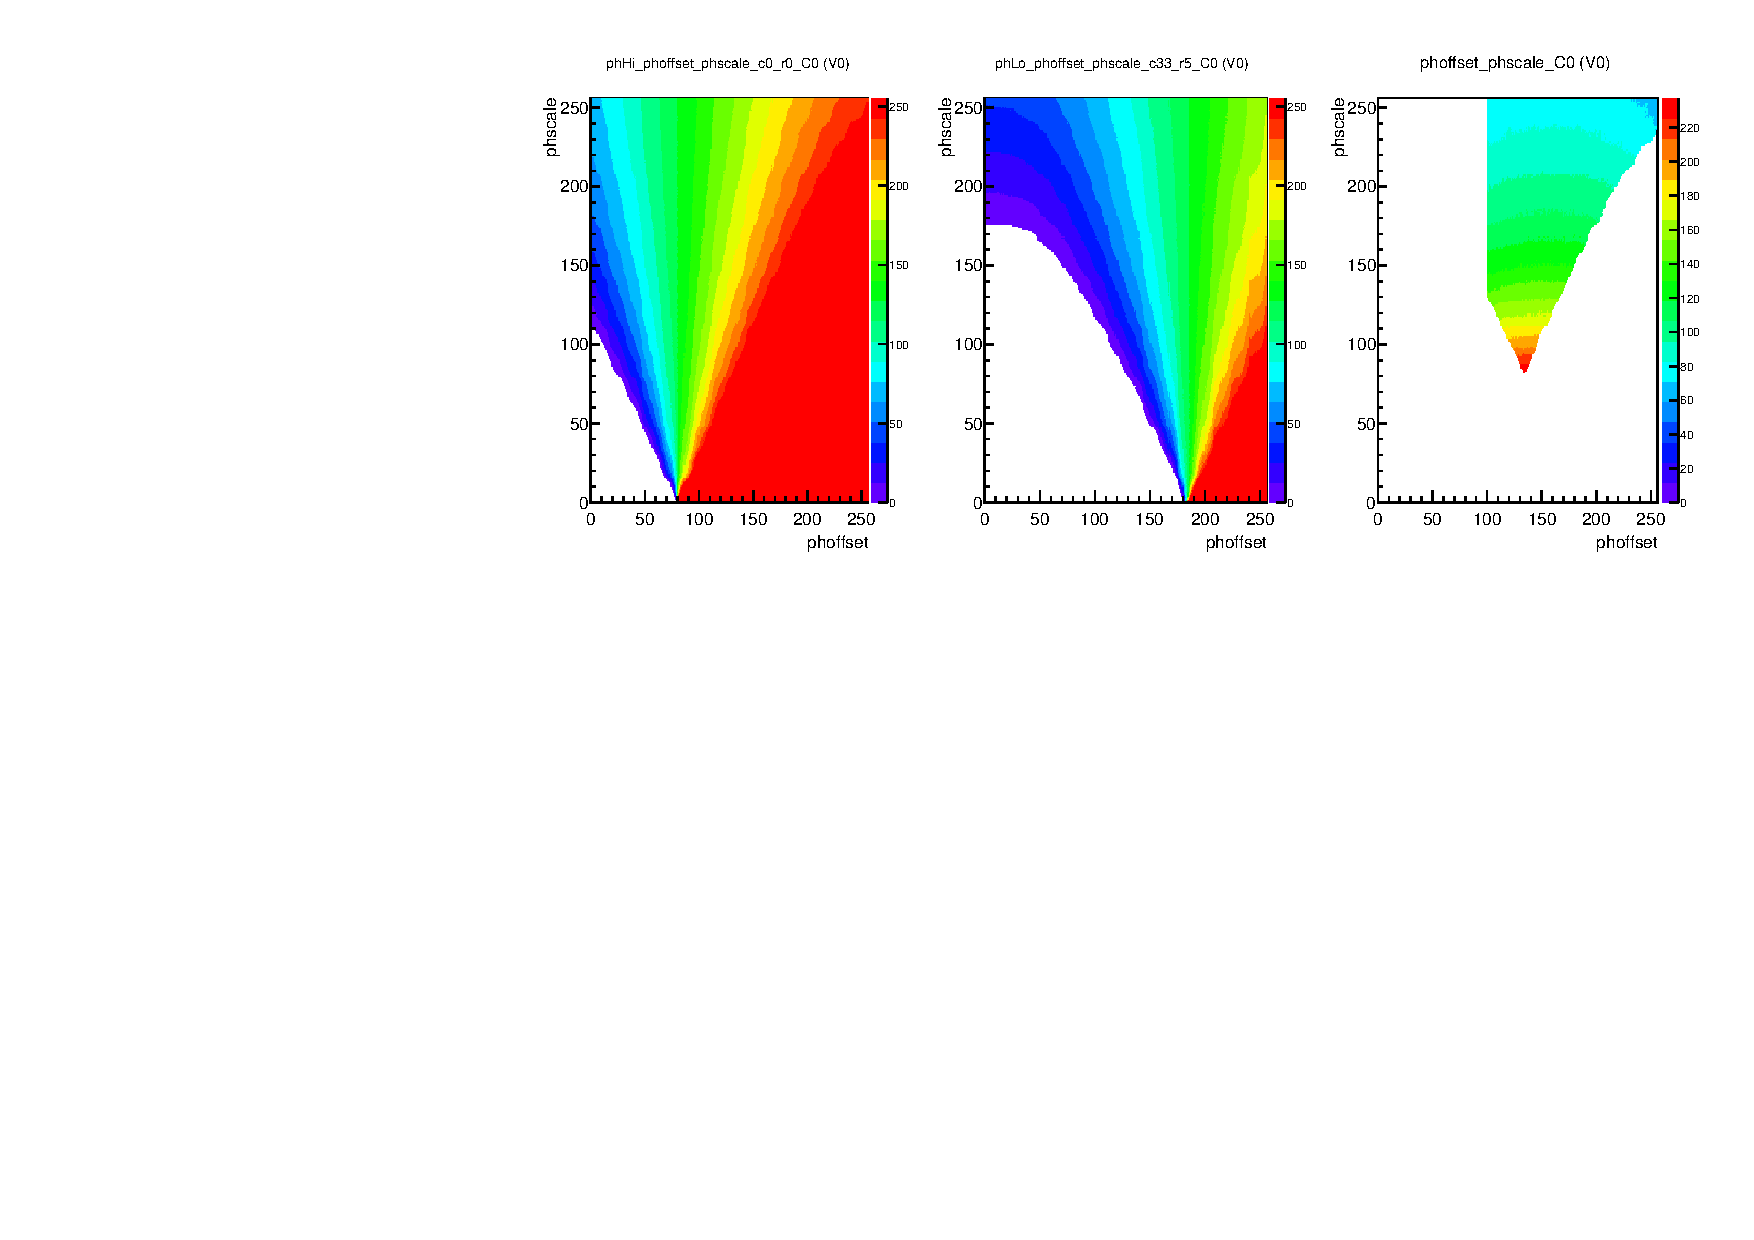
\includegraphics[height=6.0cm]{../doc/usermanual/fig/phoptimization-illustration.pdf}}
  \end{picture}
  \caption{Illustration of the \ph\ optimization algorithm. (left)
    Scan for \vcal=255 of \phscale\ vs.~\phoffset\ for pixel (0,0) which is chosen
    because the entire chip is in saturation (cf.~Fig.~\ref{f:phmap}
    right). (middle) The corresponding scan for pixel (33,5) for
    \vcal=10. (left) The difference between the left and middle
    plot. The shape of the contour is due to requirements that the
    maximum \ph\ be less than 255 (= {\tt phmax}), that the minimum \ph be larger
    than 10 (={\tt phmin}), and that {\tt phoffsetmin} be larger than 100. }
  \label{f:phoptillustration}
 \end{centering}
\end{figure}


The test parameters controlling this algorithm are summarized (in
parenthesis the default values are provided) in the following.
\begin{itemize}
  \item {\tt vcallow (= 10, high range)} set the charge injection
    when determining the \ph\ in the small signal range. It is used to
    determine to the pixel (per ROC) with the smallest \ph\ value. It
    should be noted that {\tt vcallow} should be above the minimum
    threshold to which the ROC has been trimmed (beforehand!).
  \item {\tt vcalhigh (= 255, high range)} set the charge injection
    when determining the \ph\ in the large signal range. It is used to
    determine to the pixel (per ROC) with the largest \ph\ value.
  \item {\tt phscalemin (= 50)} minimum setting for
    \phscale. Parameters below this value are not considered as valid
    points.
  \item {\tt phoffsetmin (= 100)} minimum setting for
    \phoffset. Parameters below this value are not considered as valid
    points.
  \item {\tt phmin (= 2)} minimum \ph\ acceptable for the pixel with
    the smallest \ph\ response with a calibration pulse of {\tt vcallow}.
  \item {\tt phmax (= 250)} maximum \ph\ acceptable for the pixel with
    the largest \ph\ response with a calibration pulse of {\tt vcalhigh}.
\end{itemize}
The dependence of the optimization procedure on the exact values of
{\tt phmin}  and {\tt phmax} is not large, as illustrated in
Fig.~\ref{f:phopt-phmin-phmax}.

\begin{figure}[!htb]
 \begin{centering}
  \unitlength1.0cm % coordinates in cm
  \begin{picture}(15.0, 6.0)
    \put(-0.5, 0.){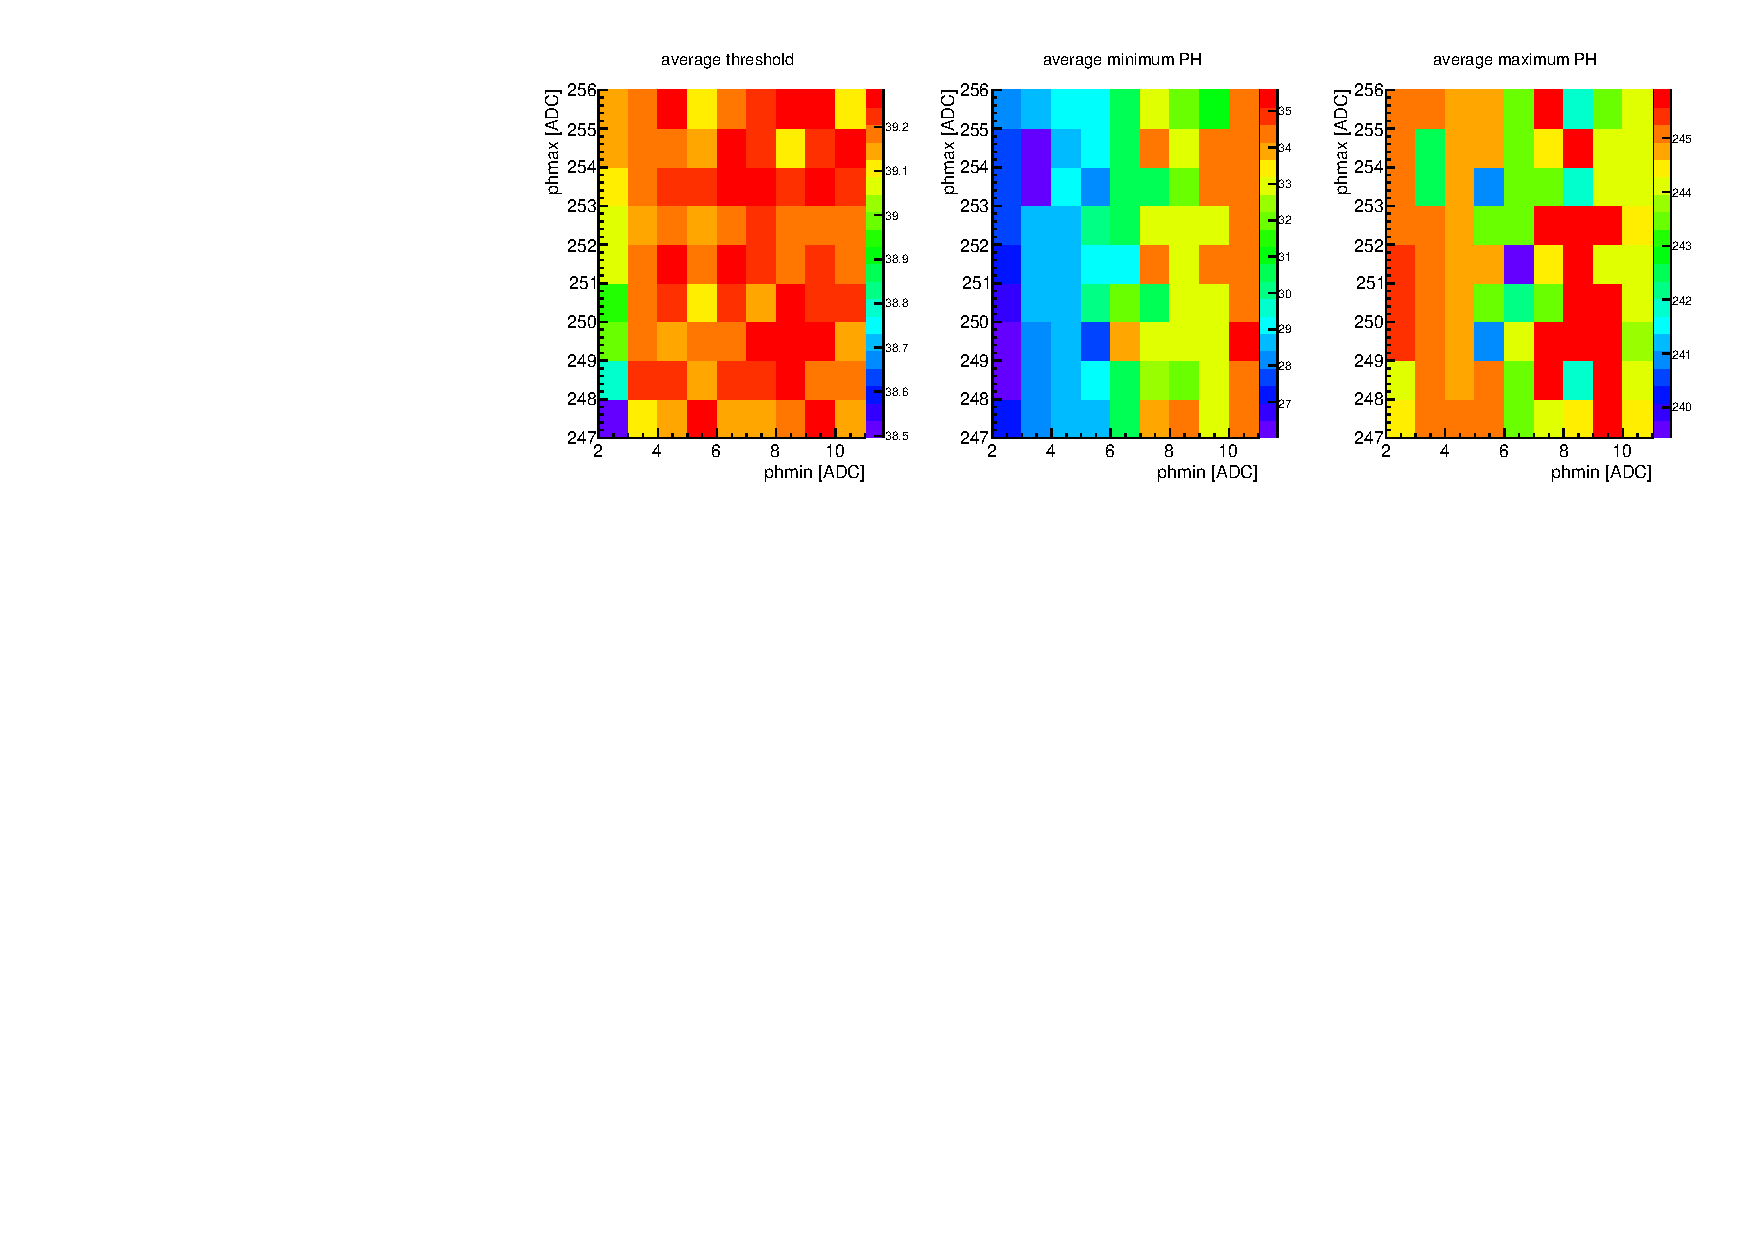
\includegraphics[height=6.0cm]{../doc/usermanual/fig/phValidation-2dscans-phmin-phmax.pdf}}
  \end{picture}
  \caption{Dependence of the \ph\ optimization on  {\tt phmin}  and
    {\tt phmax}, determined with the \gptest. The top plot shows the
    average threshold (for a ROC trimmed to \vcal=35, low range). The
    bottom left plots shows the average of the minimum
    \ph\ distribution, the right plots show the average of the maximum
    \ph\ distribution. Note the compressed $z$-axis scale for the
    lower two plots.}
  \label{f:phopt-phmin-phmax}
 \end{centering}
\end{figure}

As validation of the optimization procedure, the \ph\ distribution for
the small and large \vcal\ charge injection are provided in
Fig.~\ref{f:phvalidation}.

\begin{figure}[!htb]
 \begin{centering}
  \unitlength1.0cm % coordinates in cm
  \begin{picture}(15.0,6.0)
    \put(2, 0.){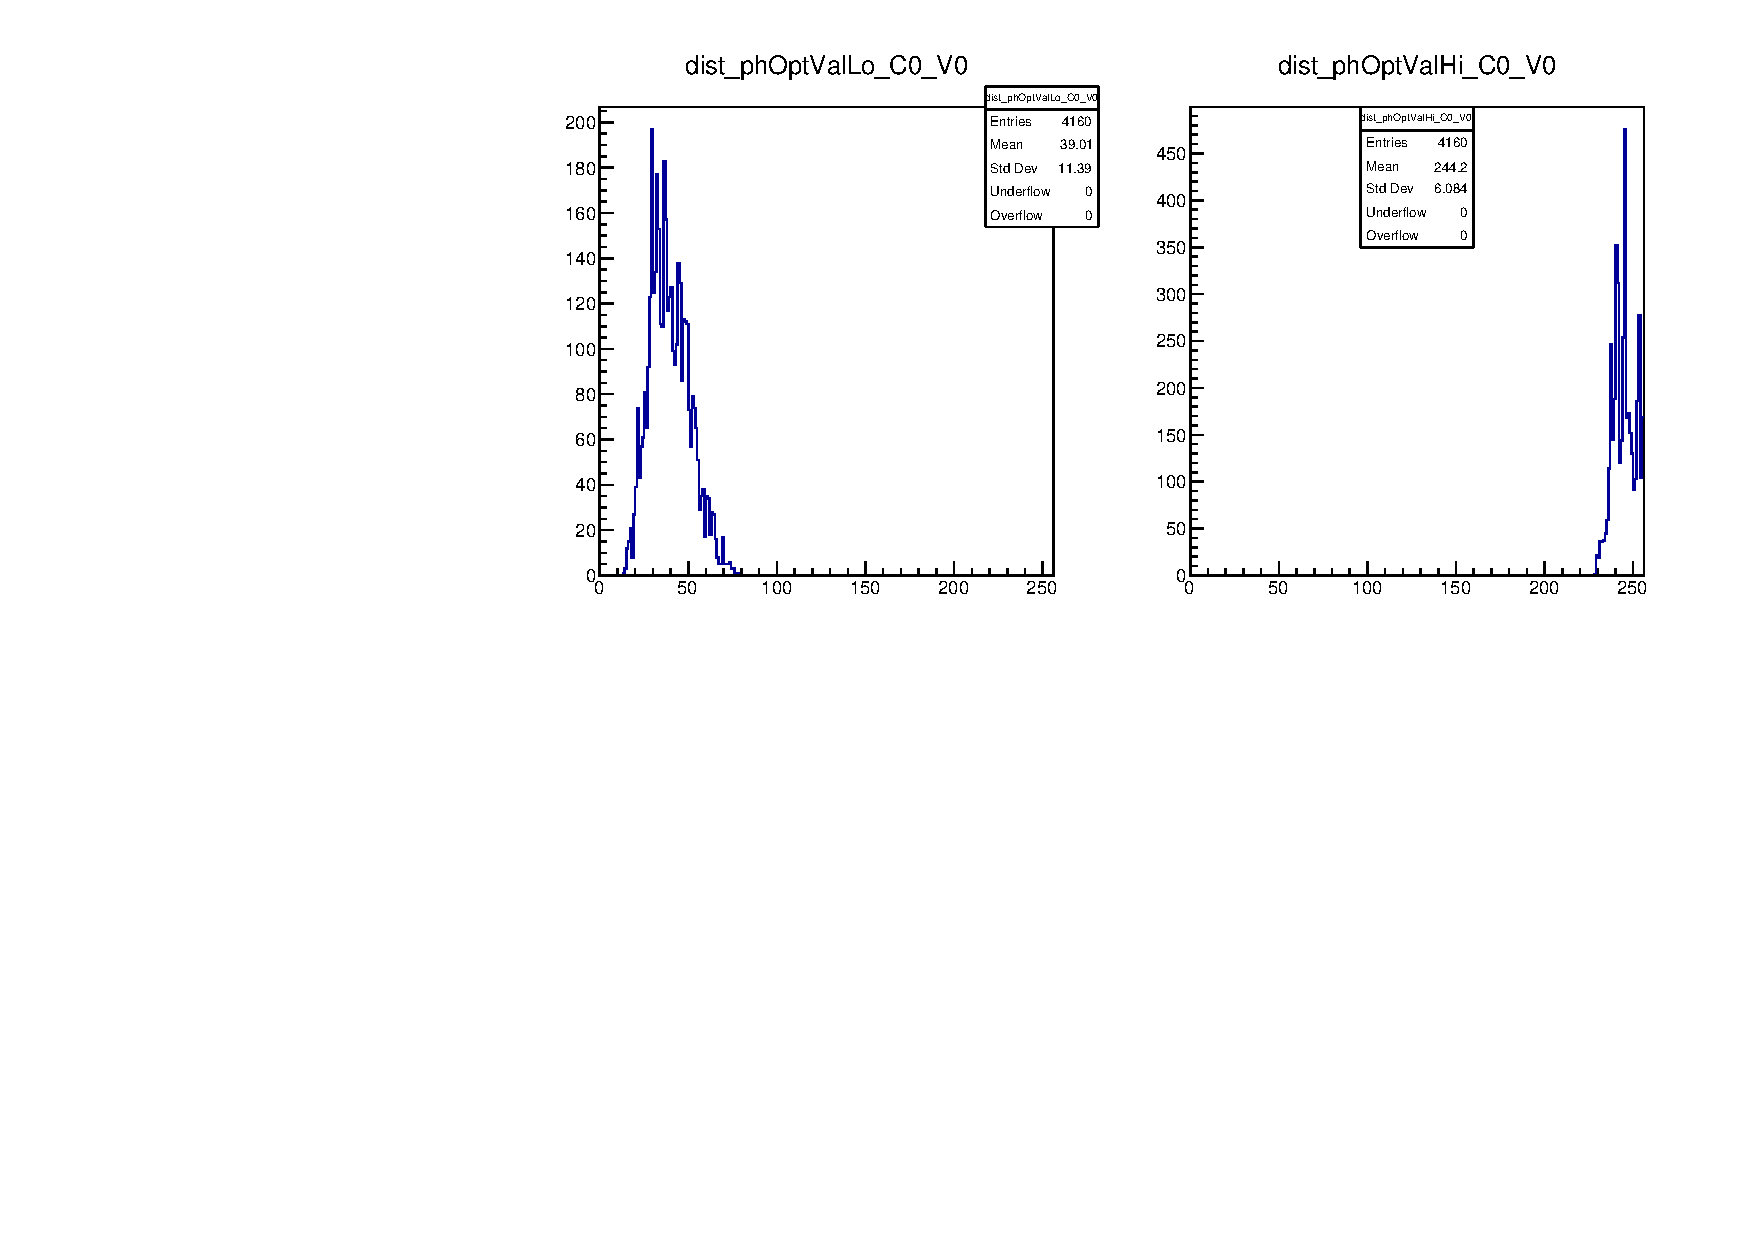
\includegraphics[height=6.0cm]{../doc/usermanual/fig/phoptimization-validation.pdf}}
  \end{picture}
  \caption{Validation of the {\tt\phtest:optimize} test: distribution
    of the low-\vcal\ charge injection (left) and the
    large-\vcal\ charge injection test.  }
  \label{f:phvalidation}
 \end{centering}
\end{figure}


It should be noted that the optimization results are not well defined
if the test is run with suboptimal parameters on untrimmed
\rocs\ (especially if the parameter {\tt vcallow} is below the
\vcal\ threshold for all pixels).

% ----------------------------------------------------------------------
\subsection{VCal calibration}
\label{ss:vcalcal}

% ----------------------------------------------------------------------
\subsection{High-rate test}
\label{ss:hrmaps}

% ----------------------------------------------------------------------
\section{User tests}
\label{s:usertests}
% ----------------------------------------------------------------------
It is straightforward to add your own tests to \pxar: you need to
write the source code and provide the configuration for
\testparameters. 
\begin{itemize}
\item The source code for all user tests are is located in
  \usertests. It is recommended that the name of your class starts
  with {\tt PixTest}. Provide the class definition in a header file ,
  whose name (without the extension {\tt .hh}) corresponds to the
  class name. Provide the implementation in a source file with
  extension {\tt .cc}. Following these recommendations allows that the
  `glob' in {\tt usertests/CMakeLists.txt} file picks up all user test classes in
  \usertests, and there is no need to manually insert your filenames
  into {\tt usertests/CMakeLists.txt}. 
\item To instantiate your test class in the GUI, and to provide the
  initial configuration of the test parameters, provide a section for
  \testparameters. 
\end{itemize}
After inserting the header and implementation files into \usertests,
go to your build directory, re-run the \cmake command, and
compile. The \cmake step will (re)build the {\tt
  pxar/usertests/PixUserTestFactory.cc} file, which will make your
test class visible, for instance in the GUI.


\end{document}
